%!TEX root = ../thesis.tex
%*******************************************************************************
%****************************** Fourth Chapter **********************************
%*******************************************************************************
\chapter{Results}

% **************************** Define Graphics Path **************************

\graphicspath{{Chapter4/Figs/Vector/}{Chapter4/Figs/}}
\section{Non-Parametric}
Non-parametric equations have the benefit of not requiring the minimisation function.
\subsection{Monte Carlo}
Using a test sample size
\begin{figure}
    \begin{center}
        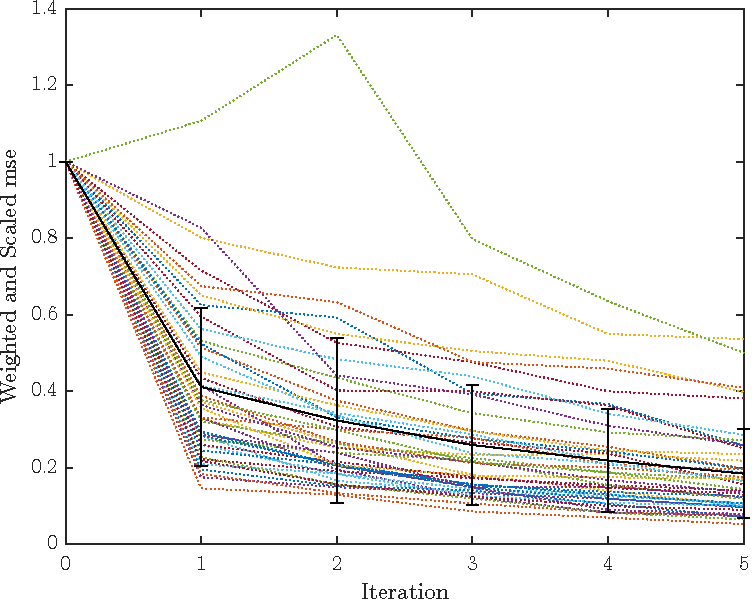
\includegraphics{dumb1.pdf}
        \caption[Batch Cluster Sampling]{}
    \end{center}
\end{figure}

\subsection{Uncertainty Sampling}
\begin{figure}
    \begin{center}
        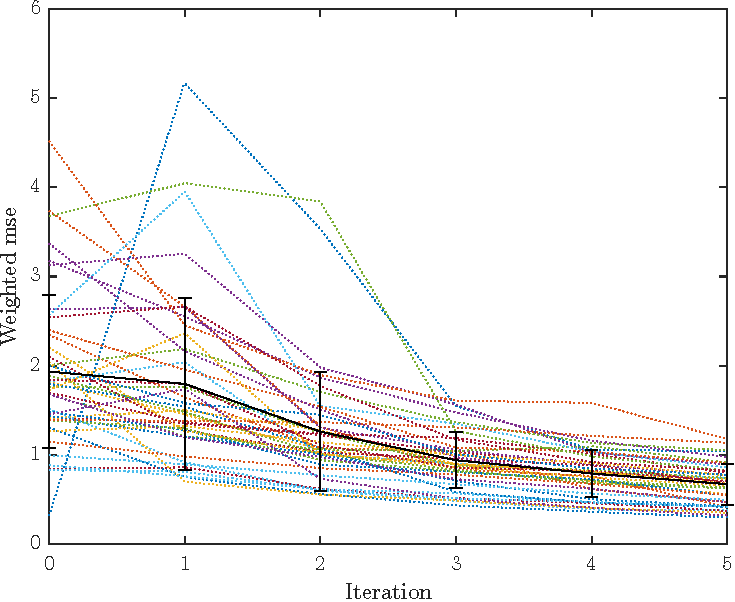
\includegraphics{rod1.pdf}
        \caption[Batch Cluster Sampling]{}
    \end{center}
\end{figure}

\section{Parametric}
\blindtext[1]
\section{Second Part}
\blindtext[3]
\section{Special Case: COVID-19}